\section{Overview of Approach} \label{Sec:approach}

\begin{figure*}
\centering
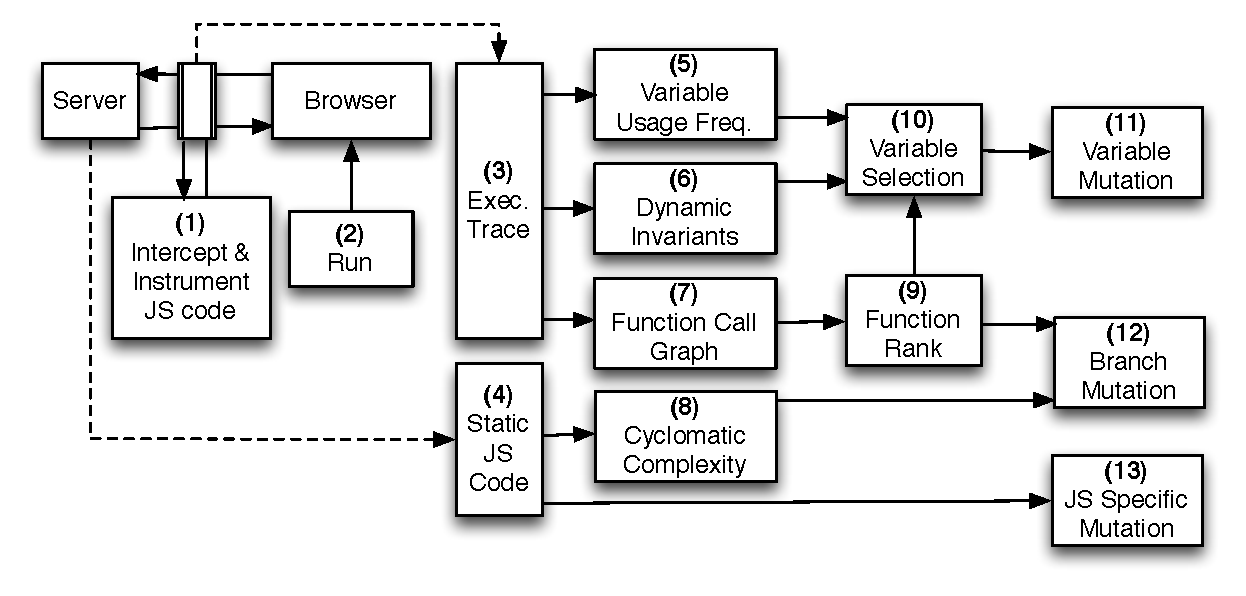
\includegraphics[width=0.7\hsize]{fig/approach-view}
\mycaption{Overview of our mutation testing approach.}
\vspace{-0.1in} 
\label{Fig:mutation}
\end{figure*}


An  overview of our mutation testing technique is depicted in \figref{mutation}. Our main goal is to narrow the scope of the mutation process to parts of the code that affect the application's behaviour, and/or are more likely  to be error-prone and difficult to test. We describe our approach below.  The numbers below in parentheses correspond to those in the boxes of \figref{mutation}.

In the first part of our approach, we
(1) intercept the \javascript code of a given web application, by setting up a  proxy between the server and the browser, and instrument the code, 
(2) execute the 
%software under test (SUT) to produce execution traces.
instrumented program by either crawling the application automatically, or by running the existing test suite (or a combination of the two), and (3) gather detailed execution traces of the application under test. 

We then extract the following pieces of information from the 
execution traces, namely (5) variable usage frequency, 
(6) dynamic invariants, and (7) the functions' call frequency.
In addition to dynamically inferred information from the execution traces, 
we also construct the function call graph of the application by incorporating both static and dynamic information.
%Because we use the execution trace, we can extract the precise call graph, 
%as opposed to a static approximation. 

Using the function call graph and the dynamic call frequencies, we (9) rank the program's functions in terms of their relative importance from the application's behaviour point of view. The higher a function's ranking, the more likely it will be selected for mutation in our approach.

Further, within the highly ranked functions, our technique (10)  identifies variables 
that have a significant impact on the function's outcome based on the 
usage frequency and dynamic invariants extracted from the execution traces, 
and (11) selectively mutates only those variables to reduce the likelihood of equivalent mutants. 
%\karthik{I made variable mutation box as box 11 ?}
%Our technique  based on the dynamic invariants

%\karthik{I changed the figure to add an arc leading from the cyclomatic complexity and function rank box to the branch mutation} 
In addition to variables, our technique mutates branch conditions, including loops. %and conditional statements. 
%based on the cyclomatic complexity (also known as structural complexity) of the \javascript code.
Functions with high cyclomatic complexity are known to be more error-prone and challenging to test \cite{basili:tse96, nagappan:icse06},  as the tester needs to detect and 
exercise all the different paths of the function. 
We therefore (4) statically analyze
the \javascript code of the web application, and (8) measure its
cyclomatic complexity. To perform branch mutation (12), we target the highly ranked functions (selected in 9) that also exhibit high cyclomatic complexity.
%\karthik{Can we number the branch mutation box as 12 ?}.

%\karthik{Can we number the ]javascript mutation box as 13 ?}
In addition to the generic mutation operators, our technique considers (13) a number of \javascript
specific mutation operators, based on an investigation of common errors made by web programmers. %as well as DOM specific mutations  at the \javascript code level.
These specific operators are applied without any ranking or selection process. %and do not take into account the dynamic execution characteristics of the application. 

%Our mutation technique is composed of the following main steps: 
%(1) ranking functions , (2) ranking variables, and (3) mutation process, which applies the mutation operators to the code.  
%In the following three sections, we describe each step in detail.
Our overall guided mutation testing algorithm is presented in \algref{mutationAlgo}.
In the following three sections, we describe in detail our technique for ranking functions 
(\secref{ranking}), ranking and selecting variables (Section \ref{variable-ranking}), and performing the actual mutations, including the mutation operators (\secref{mutation-process}). 


\section{Ranking Functions} \label{Sec:ranking}
In this section, we present our function ranking approach, which is used for selective variable and branch mutation.
%As it is shown in \figref{mutation}, 

 
\subsection{Ranking Functions for Variable Mutation}
\label{Sec:rankfunc-var}
%To rank functions for selective \emph{variable} mutation, we propose a new metric called $FunctionRank$. 

%
%In order to detect critical functions, that are more likely to exhibit severe bugs,
In order to rank and select functions for  variable mutation generation,  we propose a new metric called $FunctionRank$, which is based on $PageRank$  \cite{brin:cnis98}, but takes dynamic function calls into account. As such, $FunctionRank$ measures the relative importance of each function at runtime. %We compute $FunctionRank$ on the call graph of the application. 
To calculate this metric, we use a function call graph inferred from a combination of static and dynamic analysis (line 6 in \algref{mutationAlgo}). Our insight is that the more a function is used, the higher its impact will be on the application's behaviour. As such, we assign functions that are highly ranked, a higher selection probability for mutation.

\headbf{Function Call Graph} \label{Sec:functionCallGraph}
To create a function call graph, we use dynamic as well as static analysis.
We instrument the application to record the callee functions per call, which are  encountered during program execution.
However, the obtained dynamic call graph may be incomplete due to the presence of uncovered functions during the program execution.
Therefore, to achieve a more complete function call graph, we further infer the static call graph through static analysis. 
We detect the following types of function calls in our static analysis of the application's code:

\begin{enumerate}
 \item Regular function calls \eg~\code{foo()};
 \item Method calls \eg~\code{obj.foo()};
 \item Constructors \eg~\code{new foo()};
 \item Function handlers \eg~\code{e.click(foo)};
 \item Anonymous functions called by either a variable or an object property where the anonymous function is saved.
\end{enumerate}

We enhance our dynamically inferred call graph of the executed functions by merging the graph with the statically obtained call graph containing uncovered functions. 
Note that constructing function call graph for the \javascript applications using static analysis is often unsound due to highly dynamic nature of the \javascript language. In \javascript functions can be called through dynamic property access (e.g., \code{array[func]}). They can be stored in object properties with different names, and properties can be dynamically added or removed. Moreover, \javascript functions are first class meaning that they can be passed as parameters. While static program analysis cannot reason about such dynamic function calls in \javascript applications, relying on pure dynamic analysis can also lead to an incomplete call graph because of the unexecuted functions that are part of the uncovered code at run-time. Therefore, in our approach we choose to first construct our function call graph based on dynamic information obtained during the execution, and then make use of static analysis for those functions that are remained uncovered during the execution. 
%\karthik{So do we calculate the union of the two graphs ? How is this more accurate than just the static graph ?}

\headbf{Dynamic Call Frequencies} \label{Sec:dynamicCallFreq}
While the caller-callee edges in the call graph are constructed through static analysis of the application's code, the call frequency for each function is inferred dynamically from the execution traces (line 3 in \algref{mutationAlgo}).
The call graph also contains a mock node, called $main$ function, which represents the entire code block in the global scope, \ie global variables and statements that are not part of any particular function.
The $main$ node does not correspond to any function in the program.
In addition, function event handlers, which are executed as a result of triggering an event, are linked to the $main$ node in our dynamic call graph.

\IncMargin{0.5em}
\begin{algorithm}[t]
{\scriptsize
\SetKwInOut{Input}{input}\SetKwInOut{Output}{output}
\Input{A Web application $App$, the maximum number of variable mutations $MaxVarMut$ and branch mutations $MaxBrnMut$}
\Output{The mutated versions of application \textit{Mutants}}
\BlankLine
\nl \textit{App} $\leftarrow \textsc{Instrument}(App)$ \\
\Begin {
\nl \textit{trace} $\leftarrow \textsc{CollectTrace}(App)$ \\
\nl $\{callFrq_{f_{i,j}}, varUsgFrq_{f_{i}}, invars_{f_{i}}\}$ $\leftarrow \textsc{GetRequiredInfo}(\textit{trace})$\\
\nl $l=m=0$\\
\nl \While {$l<MaxVarMut$}{
\nl 	$\{FR(f_i)_{i=0}^n\}$ $\leftarrow \textsc{FunctionRank}(callGraph, callFrq_{f_{i,j}})$\\
\nl 	\textit{mutF} $\leftarrow \textsc{SelectFunc}(\big(FR(f_i)\big)_{i=0}^n)$\\
\nl 	$\alpha$ $\leftarrow$ $\frac{1}{1-ReadVar_{f_{i}}}$\\
\nl 	$candidVars_{mutF}$ $\leftarrow invars_{mutF} \cup \{v_i|varUsgFrq_{mutF}(v_i)>\alpha\}$\\
\nl 	$\{pr(v_i\in candidVars_{mutF})\}$ $\leftarrow \frac{1}{|candidVars_{mutF}|}$\\
\nl 	\textit{mutVar} $\leftarrow \textsc{SelectVar}(candidVars_{mutF}, pr(v_i))$ \\
\nl 	$mutant_l \leftarrow \textsc{VariableMutation}(mutF,mutVar,varMutOps)$\\ 	
\nl 	$l++$\\
}
\nl \textit{varMutants} $\leftarrow \bigcup mutant_{l=1}^{MaxVarMut}$\\
\nl \While {$m<MaxBrnMut$}{
\nl 	$\{pr(f_i)_{i=0}^n\}$ $\leftarrow \frac{fcc(f_i) \times FR(f_i)}{\sum _{j=1}^{n} fcc(f_i) \times FR(f_i)}$\\
\nl 	\textit{mutF} $\leftarrow \textsc{SelectFunc}(\big(pr(f_i)\big)_{i=0}^n)$\\  
\nl 	\textit{mutBrn} $\leftarrow \textsc{SelectRandomBrn}(mutF)$ \\
\nl 	$mutant_m \leftarrow \textsc{BranchMutation}(mutBrn,brnMutOps)$\\
\nl 	$m++$\\
}
\nl \textit{brnMutants} $\leftarrow \bigcup mutant_{m=1}^{MaxBrnMut}$\\
\nl \textit{Mutants} $\leftarrow varMutants \cup brnMutants$\\
\nl return \textit{Mutants}
}
\caption{Guided Mutation Algorithm.}
\label{Alg:mutationAlgo}
}
\end{algorithm}
%\DecMargin{lem}

\headbf{The FunctionRank Metric} 
%\label{Sec:functionRankMetric} \ali{this is not a section so labels won't work}
The original $PageRank$ algorithm \cite{brin:cnis98} assumes that for a given vertex, 
the probability of following all outgoing edges is identical, and hence
all edges have the same weight. For $FunctionRank$, 
we instead apply edge weights proportional to the dynamic call frequencies of the functions.  % obtained from  execution traces. %(by using a relaxed form of the original formula). 
%However, the $PageRank$ formula requires that
%the weights on the outgoing edges sum to 1. 
%Therefore, we need to normalize the edge weights from 
%each function in our formula. 

Let $l(f_{j},f_{i})$ be the weight assigned to 
edge $(f_{j},f_{i})$, in which function $i$ is called by function $j$. 
We compute $l$ by measuring the frequency of function $j$ calling $i$ 
during the execution.  We assign a frequency of 1 to edges directing to unexecuted functions.
%We consider the number of times that function $i$ calls an unexecuted function during the application's run is equal to one. 
The $FunctionRank$ metric is calculated as:

\begin{equation}
FR(f_i)=\sum _{j\in M(f_i)} {FR(f_j)\times l(f_j,f_i)},
\label{functionRankFormula}
\end{equation}
where, $FR(f_i)$ is the $FunctionRank$ value of function $i$, $l(f_j,f_i)$ is
the frequency of calls from function $j$ to $i$, and $M(f_i)$ is the set of
functions that call function $i$%., and $n$ is the total number of functions.

The initial $PageRank$ metric requires 
the sum of weights on the outgoing edges to be 1.
Therefore, to solve equation \ref{functionRankFormula}, we need to normalize the edge weights from 
each function in our formula such that for each $i$,
$\sum _{j=1}^{n} {l(f_i,f_j)}=1$.   
To preserve the impact value of call frequencies on edges when compared globally in the graph,
we normalize $l(f_i,f_j)$ over the sum of weights on all edges. Since outgoing edges from
function $f_i$ should sum to 1, an extra node called $fakeNode$ is added to the graph. Note that the extra $fakeNode$ is different from the mock $main$ node added earlier. $fakeNode$ contains an incoming edge from $f_i$, where:
%\karthik{We should make it clear that the fakeNode is different from the mock node added earlier}

\begin{equation}
 l(f_i,fakeNode)=1-\sum _{j=1}^{n} {l(f_i,f_j)}
 \end{equation}

Functions with no calls are also linked to the $fakeNode$ through an outgoing edge with weight 1.

A recursive function is represented by a self-loop to the recursive node in the function call graph.
The original $PageRank$ does not allow for self-loop nodes (\ie a web page with a link to itself).
Self-loop to a node infinitely increases its rank without changing the relative rank of the other
nodes. Therefore, such nodes are disregarded in the original $PageRank$ formula. 
However, recursive functions are inherently important as they are error-prone and difficult to debug, and they can easily propagate a fault into higher level functions. To incorporate recursive functions in our analysis, we break the self-loop to a recursive function $Recf_i$ by replacing the function with nodes $f_i$ and $f_{ci}$ in the function call graph. We further add an edge $l(f_i,f_{ci})$, where $l$ is the call frequency associated with the recursive call. 
All functions that are called by $Recf_i$ will get an incoming edge from the added node $f_{ci}$.  
This way,  all the functions called by $Recf_i$ are now linked to $f_{ci}$ (and indirectly linked to $f_i$).
After the $FunctionRank$ metric is computed over all functions, we assign the new $FunctionRank$ value of the recursive node as follows: 
$FR(Recf_i)=FR(f_i)+FR(f_{ci})$, where $FR(Recf_i)$ is the new $FunctionRank$ value assigned to the recursive function $Recf_i$. %\ali{I don't understand this previous paragraph. We need a better explanation of what we are doing and why we are doing it.}

\begin{figure*} [tp]
\centering
\subfloat[Call graph with call numbers.]{\label{Fig:origGraph}
       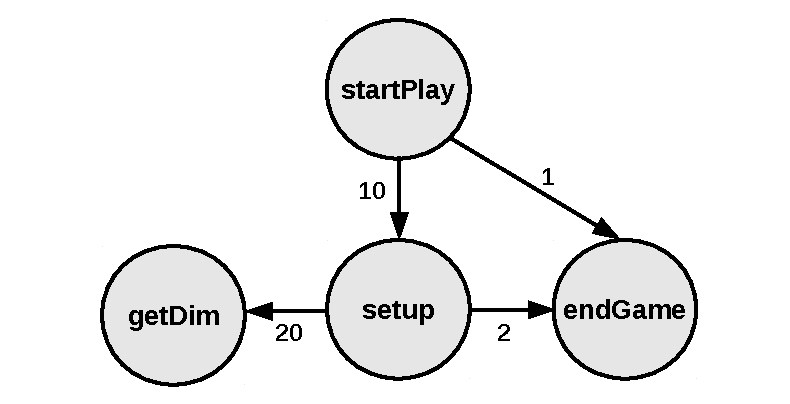
\includegraphics[width=.6\textwidth]{fig/exampleGraph0}}
\subfloat[Call graph with call frequencies.]{\label{Fig:modifGraph}
       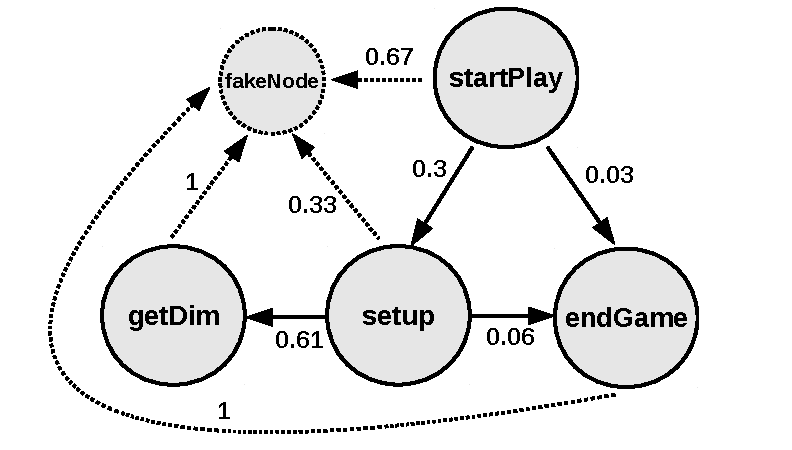
\includegraphics[width=.6\textwidth]{fig/exampleGraph}}
\vspace{0.2in}             
\caption{Call graph of the running example.}
\label{Fig:exampleGraph}
\end{figure*}
 
%\begin{figure}
%\centering
%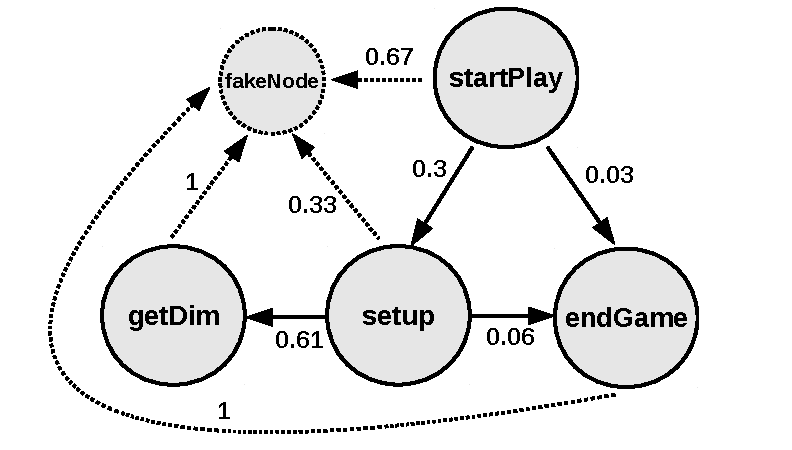
\includegraphics[width=0.8\hsize]{fig/exampleGraph}
%\vspace{0.15in} 
%\mycaption{Call graph of the running example.}
%\label{Fig:exampleGraph}
%\vspace{-0.1in} 
We initially assign equal $FunctionRank$ values to all nodes in \ref{functionRankFormula}.%\end{figure}
The calculation of $FunctionRank$ is performed recursively, %\ali{isn't it recursivly?},
until the values converge. 
Thus,  the $FunctionRank$ of a function $i$ depends on:

\begin{enumerate}
\item the number of functions that call $i$;
\item the $FunctionRank$ values of the functions that call $i$ (incoming edges);
\item the number of dynamic calls to $i$.
\end{enumerate}

Hence, a function that is called by several functions with high $FunctionRank$s
and high call frequencies receives a high $FunctionRank$ itself.

At the end of the process, the extra function $fakeNode$ is removed and the $FunctionRank$ value of all other functions is multiplied by $\frac{1}{1-FR_{fakeNode}}$, where $FR_{fakeNode}$ is the calculated 
$FunctionRank$ of $fakeNode$. 

Overall, our approach assigns each function a $FunctionRank$  value between 0 and 1.
These values are used to rank and select functions for variable mutation (lines 6-7 in \algref{mutationAlgo}). 
The higher the $FunctionRank$ value of a given function, the more 
likely it is to be selected for mutation. 

\figref{exampleGraph} depicts the function call graph obtained from our running example (\figref{example}). The labels on the edges of \figref{origGraph} show the
number of calls to each function in the graph. \figref{modifGraph} shows the modified graph with the extra node $fakeNode$ added to compute the normalized function call frequency  values.
%The labels on the edges of \figref{modifGraph} are edge weights calculated according to the function call frequency. 
In our example, assuming that the number of \code{div} elements is 20 (line 3 in \figref{example}), \code{setup} will be called 20 times and \code{endGame} will be called once (lines 4 and 6). Now, assume that the number of DOM elements with the class name specified as the input to function \code{setup} varies each time \code{setup} is called (line 10) such that two elements have a length of zero and the total length of the rest is  20. Then, function \code{endGame} is called twice (in line 12) when the length of such elements is zero, and \code{getDim} is called 20 times in total (line 14). Therefore, the call frequencies of functions \code{setup} and
\code{endGame} become 0.3 and 0.03 respectively when they are called by \code{startPlay} in lines 4 and 6.
Similarly, the call frequencies of \code{getDim} and \code{endGame} become 0.61
and 0.06, respectively, when called by \code{setup}. 

Note that if the weight on an outgoing edge of a given function is simply normalized over the sum of the weights on all the outgoing edges of that function, then the call frequencies  
for both \code{setup} and \code{getDim} become 0.91 when they are called by \code{startPlay} and \code{setup}, respectively. However, as shown in \figref{origGraph} the number of times that function \code{getDim} is called is twice that of \code{setup}. To obtain a realistic normalization, we have introduced the $fakeNode$, as shown in \figref{modifGraph}.
 
%Using equation \ref{functionRankFormula}, we are able to calculate $FunctionRank$ values associated with each of the functions in the graph shown in \figref{modifGraph}. 
\tabref{fr-pr-table} shows the computed 
$FunctionRank$ values, using equation \ref{functionRankFormula}, for each function of the running example. The values are presented as percentages. \code{getDim} achieves the highest $FunctionRank$ because of the relatively high values of both the incoming edge weight (where \code{getDim} is called by \code{setup} in line 14 in \figref{example}), and the $FunctionRank$ of its caller node, \code{setup}.
These ranking values are used as probability values for selecting a function for mutation. 

To illustrate the advantage of $FunctionRank$, we show the same calculation using the traditional $PageRank$ metric, i.e., without considering dynamic edge weights. As shown in \tabref{fr-pr-table}, \code{endGame} obtains the highest ranking using $PageRank$. However, this function has not been used extensively during the application execution, and hence has only limited impact on the behaviour of the application. 
In contrast, when $FunctionRank$ is used, \code{endGame} falls to the third place, and is hence less likely to be chosen for mutation. 

%$FR(\code{endGame})<\frac{1}{2}FR(\code{getDim})$. Thus, the probability of choosing
%\code{getDim} for mutation is considerably higher than \code{endGame}. 

\begin{table}
%\vspace{5pt}
        \caption{Computed $FunctionRank$ and $PageRank$ for the running example.}
{\scriptsize
   
       \begin{center}
      %  \subtable[Experimental subjects and the corresponding exploration data]
            {
          \begin{tabular}{l|c|c} \hline
\thead{Function Name} & \thead{FunctionRank (\%)} & \thead{PageRank (\%)} \\  \hline \hline

  \code{getDim} & 34.5 & 27.0 \\ \hline
  \code{setup} & 25.0 & 23.0 \\ \hline
  \code{endGame} & 21.3 & 34.6 \\ \hline
  \code{startPlay} & 19.2 & 15.4 \\ \hline

\hline \end{tabular}\centering
            }

\label{Table:fr-pr-table}
\end{center}
}  
\vspace{-0.1in} 
\end{table}

\subsection{Ranking Functions for Branch Mutation}
\label{Sec:funcrank-branch}
%In addition to calculating $FunctionRank$ based on the dynamic analysis of application, we also take the structural complexity of functions into account in order to mutate branch statements of the program. 
To rank functions for \emph{branch} mutation, in addition to the $FunctionRank$, we take the cyclomatic complexity of the functions into account (lines 16--17 in \algref{mutationAlgo}).

%As mentioned before, we use the cyclomatic complexity of  a function in addition to its $FunctionRank$ to select functions for branch mutation (lines 16-17 in \algref{mutationAlgo}). 
%Cyclomatic complexity is one of the widely used metrics to measure the structural complexity of a function \cite{mccabe:tse76}.
The cyclomatic complexity measures the number of linearly independent paths through a program's source code~\cite{mccabe:tse76}. By using this metric, we aim to 
concentrate the branch mutation testing effort on the functions that are error-prone and harder to test.

We measure the cyclomatic complexity frequency of each function through static analysis of the code. Let $fcc(f_i)$ be the cyclomatic complexity frequency measured for function $f_i$, then $fcc(f_i)=\frac{cc(f_i)}{\sum _{j=1}^{n} cc(f_j)}$,  
where $cc(f_i)$ is the cyclomatic complexity of function $f_i$, given that the total number of functions in the application
is equal to $n$.

We compute the probability of choosing a function $f_i$ for branch mutation using the previously measured $FunctionRank$ ($FR(f_i)$) as well as the cyclomatic complexity frequency ($fcc(f_i)$). Let $p(f_i)$ be the probability of selecting a function $f_i$ for branch mutation, then:

\begin{equation}
p(f_i)= \frac{fcc(f_i) \times FR(f_i)}{\sum _{j=1}^{n} fcc(f_j) \times FR(f_j)},
\label{fr-cc-formula}
\end{equation} 
where $fcc(f_i)$ is the cyclomatic complexity frequency measured for function $f_i$, and $n$ is the total number of  functions.

\begin{table}
%\vspace{5pt}
        \caption{Ranking functions for branch mutation (running example).}
{\scriptsize
   
       \begin{center}
      %  \subtable[Experimental subjects and the corresponding exploration data]
            {
          \begin{tabular}{l|c|c|c} \hline
\thead{Function Name} & \thead{cc} & \thead{fcc} & \thead{Selection Probability ($p$)} \\  \hline \hline

  getDim & 4 & 0.4 & 0.51\\ \hline
  setup & 3 & 0.3 & 0.27\\ \hline
  startPlay & 2 & 0.2 & 0.14\\ \hline
  endGame & 1 & 0.1 & 0.08\\ \hline


 	
\hline \end{tabular}\centering
            }

\label{Table:cycloMultFr-table}
\end{center}
}  
\vspace{-0.1in} 
\end{table}
\tabref{cycloMultFr-table} shows the cyclomatic complexity, the frequency, and the function selection
probability measured for each function in our example (\figref{example}). The probabilities are obtained using equation \ref{fr-cc-formula}.
As shown in the table, \code{getDim} achieves the highest selection probability as both its $FunctionRank$ and cyclomatic complexity
are high.



\section{Ranking Variables}  \label{variable-ranking}

Applying mutations on arbitrarily chosen variables may have no effect on the semantics of the program and hence lead to equivalent mutants. Thus, in addition to functions, we  measure the importance of variables in terms of their impact on the behaviour of the function.  We target local and global variables, as well as function parameters for mutation. 

%\karthik{What are equivalent variable mutants below ?}
In order to avoid generating equivalent mutants, within each selected function, we need to mutate variables that are more likely to change the expected behaviour of the application (lines 7-12 in \algref{mutationAlgo}).
We divide such variables into two categories: 
%\begin{itemize}
%\item 
(1) those that are part of the program's dynamic invariants ($invars_{mutF}$ in line 9);
%\item 
and (2) those with high usage frequency throughout the application's execution ($varUsgFrq_{mutF}(v_i)>\alpha$ in line 9).
%\end{itemize}

\subsection{Variables Involved in Dynamic Invariants} 
A recent study \cite{schuler:issta09} showed that if a mutation violates dynamic invariants, it is very likely to be non-equivalent. 
This suggests that mutating variables that are involved in
forming invariants affects the expected behaviour of the application with a high probability.
Inspired by this finding, we infer invariants from the execution traces, as depicted in \figref{mutation}. We log variable value changes during run-time, and analyze the collected traces to infer stable dynamic invariants. The details of our \javascript invariant generation technique can be found in  \cite{mirshokraie:icwe12}. From each obtained invariant, we identify all the variables that are involved in the invariant and mark them as potential variables for mutation. 

In our running example (\figref{example}), an inferred invariant in \code{getDim} yields information about the inequality relation between function parameters \code{width} and \code{height}, e.g.,  ($width>height$). Based on this invariant, we choose
\code{width} and \code{height} as potential variables for mutation.

\subsection{Variables with High Usage Frequency} 
In addition to dynamic invariants, we  consider the impact of variables on the expected behaviour based on their dynamic usage. %(See \figref{mutation}).
We define the {\em usage frequency} of a variable as the number of times that the variable's value has been read during the execution in the scope of a given function. 
%asits usage frequency. 
Let $u(v_i)$ be the usage frequency of variable $v_i$, then $u(v_i)=\frac{r(v_i)}{\sum _{j=1}^{n} r(v_j)}$,  
where $r(v_i)$ is the number of times that the value of variable $v_i$ is read, given that the total number of variables in the scope of the function is $n$.

We identify the usage of a variable by identifying and measuring the frequency of a given variable being read in the following
scenarios: (1) variable initialization, (2) mathematical computation, (3) condition checking in conditional statements, (4) function arguments, and (5) returned value of the function. 
We assign the same level of importance to all the five scenarios. 
     
From the degree of a variable's usage frequency in the scope of a given function, we infer to what extent
the behaviour of the function relies on that variable. Leveraging the collected execution traces, 
we compute the usage frequencies in the scope of a function. 
We choose variables with usage frequencies above a threshold $\alpha$ as potential candidates for the mutation process. 
We automatically compute (line 8 in \algref{mutationAlgo}) this threshold for each function as:

\begin{equation}
\alpha = \frac{1}{ReadVariables_{f(i)}}, 
\end{equation}
where $ReadVariables_{f(i)}$ is 
the total number of variables that at some point during the execution their value have been read within function $f(i)$.

Going back to the \code{getDim} function in our running example of \figref{example}, the values of function parameters \code{width} and \code{height}, as well as the local variables \code{w} and \code{h} are read just once in lines 19 and 20, when they are involved in a  number of simple computations.
The result of the calculation is assigned to the local variable \code{v}, which then is checked as a condition for the \code{if}-\code{else} statement. \code{v} is returned from the function in either line 22 or 24,
depending on the outcome of the \code{if} statement.
In this example, variable \code{v} has the highest usage frequency since it has been used as a condition in a conditional statement as
well as the returned value of the \code{getDim} function.

Overall, we gather a list of potential variables for mutation, which are obtained based on the inferred dynamic invariants  and their usage frequency (line 9 in \algref{mutationAlgo}). Therefore, in our running example, in addition to function parameters \code{width} and \code{height}, which are part of the invariants inferred from \code{getDim}, the local variable \code{v} is also among the potential variables for the mutation process because of its high usage frequency. Note that the local variables \code{w} and \code{h} are not  in the list of candidates for variable mutation as they have a low usage frequency and are not part of any dynamic invariants directly. 
   
\section{Mutation Operators} \label{Sec:mutation-process}
%\shabnam{This section includes the information asked by Reviewer2-Q11} 
We employ generic mutation operators as well as \javascript specific mutation operators for performing mutations. 

\subsection{Generic Mutation Operators}
Our mutant generation technique is based on a single mutation at a time. Thus, we need to choose an appropriate candidate among all the potential candidates obtained from the previous ranking steps of our approach.
Our overall guided mutation process includes:
\begin{itemize}
\item Selecting a function as described in \secref{rankfunc-var} and mutating a \emph{variable} randomly selected from the list of 
potential candidates obtained from the variable ranking phase (Section \ref{variable-ranking}), 

\item Selecting a function as described in \secref{funcrank-branch} and mutating a  \emph{branch statement} selected randomly (lines 16-19 in \algref{mutationAlgo}).

\end{itemize}

\tabref{var-operator-table} shows the generic mutation operators we use for mutating global variables, local variables as well as function parameters/arguments.
\tabref{branch-operator-table} presents the operators we use for changing \code{for} loops, \code{while} loops, \code{if} and \code{switch-case} statements, as well as \code{return} statements.


% \textit{Mutants} in line 22 of \algref{mutationAlgo} contains all the variable (\textit{varMutants} in line 14) and branch mutants (\textit{brnMutants} in line 21).

%Note that the first two generic mutation operator types are applied using the ranking techniques, while the third type is applied regardless of the ranking, as these \javascript specific operators are known to be error-prone. Hence, we believe that they are important enough to be checked on their own. %by themselves.
%the function from which they are called..

%and (3) applying a number of \javascript specific operators.


\begin{table}
%\vspace{5pt}
        \caption{Generic mutation operators for variables and function parameters.}
{\scriptsize
   
       \begin{center}
      %  \subtable[Experimental subjects and the corresponding exploration data]
            {
           \begin{tabular}{p{1.4 cm}|p{6 cm}} \hline
\thead{Type}&  \thead{Mutation Operator} \\  \hline \hline

\multirow{4}{*}{Local/Global} 
  & Change the value assigned to the variable.\\ \cline{2-2} 
  \multirow{4}{*}{Variable} 
  & Remove variable declaration/initialization.\\ \cline{2-2}
  & Change the variable type by converting \code{x = number} to \code{x = string}. \\ \cline{2-2} 
  & Replace arithmetic operators ($+$, $-$, $++$, $--$, $+=$, $-=$, $/$, $*$) used for calculating and assigning a value to
the selected variable. \\ \hline  
  \multirow{2}{*}{Function} 
  \multirow{2}{*}{Parameter} 
  &  Swap parameters/arguments.\\ \cline{2-2} 
  & Remove parameters/arguments. \\  \hline


 \hline\end{tabular}\centering
            }
\label{Table:var-operator-table}
\end{center}
}  
\vspace{-0.1in} 
\end{table} 

%\headbf{Variable Mutation}
%We guide the mutant generation process towards mutating useful variables within the scope of critical functions. 

%As discussed earlier, we employ $FunctionRank$ value of a given function as a probability of selecting that function. The variable selection
%block in \figref{mutation}, targets a single variable within the scope of the selected function. It randomly chooses
%one of the potential variables among all the candidate ones obtained from the previous section. The selected $<function,variable>$ pair
%is used as an input to the variable mutation process. 
 
%In order to inject the mutation operator in the application's code, we first parse the intercepted source code into an Abstract Syntax
%Tree (AST). We apply a mutation operator on a variables, by traversing the AST in search of $<function,variables>$ pair candidates. If multiple such candidates are found, we randomly choose one of them.
%We randomly select a mutation operator from \tabref{var-operator-table}
%which shows a list of operators for mutating global variables, local variables as well as function parameters/arguments. 
%As far as local/global variables
%are concerned, these operators are able to modify the assigned values whether they are string or number literal, or obtained through 
%a mathematical computation. Removing a variable declaration (e.g. \code{var x}) or initialization (e.g. \code{var x=5}) is also part
%of these operators. In order to mutate function parameters/arguments, we either swap the ordering or remove them.

%\begin{figure}
%\centering
%\includegraphics[width=1.05\hsize]{fig/selectionBlockDiagram}
%\mycaption{Overview of the function and variable selection phase.}
%\label{Fig:selectionBlockDiagram}
%\end{figure}

\begin{table}
%\vspace{5pt}
        \caption{Generic mutation operators for branch statements.}
{\scriptsize
   
       \begin{center}
      %  \subtable[Experimental subjects and the corresponding exploration data]
            {
           \begin{tabular}{p{1.2 cm}|p{6.5 cm}} \hline
\thead{Type}&  \thead{Mutation Operator} \\  \hline \hline


  
  & Change literal values in the condition (including lower/upper bound). \\ \cline{2-2} 
\multirow{9}{*}{Loop}
\multirow{9}{*}{Statement}
  & Replace relational operators ($<$, $>$, $<=$, $>=$, $==$, $!=$, $===$, $!==$).  \\ \cline{2-2}
  & Replace logical operators ($\|$, \&\&). \\ \cline{2-2}
  & Swap consecutive nested \code{for}/\code{while}.\\  \cline{2-2}  
  & Replace arithmetic operators ($+$, $-$, $++$, $--$, $+=$, $-=$, $/$, $*$).\\  \cline{2-2}
  & Replace \code{x++}/\code{x--} with \code{++x}/\code{--x} (and vice versa). \\ \cline{2-2}  
  & Remove \code{break}/\code{continue}. \\ \hline
  
  & Change literal values in the condition.  \\ \cline{2-2} 
  \multirow{10} {*} {Conditional} 
    \multirow{10} {*} {Statement} 
  & Replace relational operators ($<$, $>$, $<=$, $>=$, $==$, $!=$, $===$, $!==$). \\ \cline{2-2}
  & Replace logical operators ($\|$, \&\&). \\ \cline{2-2}
  & Remove \code{else if} or \code{else} from the \code{if} statement. \\ \cline{2-2}
  & Change the condition value of \code{switch-case} statement. \\ \cline{2-2}
  & Remove \code{break} from \code{switch-case}. \\ \cline{2-2} 
  & Replace 0/1 with \code{false/true} (and vice versa) in the condition. \\ \hline

  \multirow{3} {*} {Return} 
    \multirow{3} {*} {Statement} 
  & Remove \code{return} statement. \\ \cline{2-2}
  & Replace \code{true} with \code{false} (and vice versa) in \code{return (true/false)}. \\ \hline


  
%  \multirow{3}{*}{DOM manipulation} & Changing the name of attribute/property  \\ \cline{2-2} 
%  & Removing the DOM manipulation methods \\ \cline{2-2}
%  & Changing the name of the element\\ \hline

\hline\end{tabular}\centering
            }
\label{Table:branch-operator-table}
\end{center}
}  
\vspace{-0.1in} 
\end{table}

%\headbf{Branch Mutation} 
%We randomly mutate a branch statement within the scope of the function obtained from the function ranking step. \tabref{branch-operator-table} presents the list of 
%operators for changing \code{for} loops, \code{while} loops as well as \code{if} and \code{switch-case} statements.

%\begin{table*}
%\vspace{5pt}
        \caption{\javascript specific mutation operators.}
{\scriptsize
   
       \begin{center}
      %  \subtable[Experimental subjects and the corresponding exploration data]
            {
          \begin{tabular}{p{12cm}|{c}} \hline
\thead{\javascript Mutation Operator} & \thead{Sources} \\  \hline \hline

   Adding/Removing the \code{var} keyword in the variable declaration. & \cite{hsuJsAntiPatterns, osmaniJsPatterns,Crockford:2008} \\ \hline
  
    Removing the \code{/g}, global search sign, from the \code{replace}. & \cite{weylJsGotchas, jsStringReplace, roy3commmonJsMistakes}\\ \hline
  
    Removing the integer base argument from the \code{parseInt}. & \cite{weylJsGotchas, burgess11jsMistakes} \\ \hline
  
 Changing \code{setTimeout(function, xsec)} to \code{setTimeout(function(), xsec)} 
(same change is applicable to \code{setInterval}). & \cite{hoPrematureInvocation, osmaniJsPatterns, gurbani13jsMistakes} \\ \hline
  
  Changing \code{setTimeout('function(x)', xsec)} to either 
\code{setTimeout(function, xsec)} or \code{setTimeout('function', xsec)} 
(same changes are applicable to \code{setInterval}). & \cite{osmaniJsPatterns, gurbani13jsMistakes} \\ \hline
  
 Replacing \code{'undefined'} with \code{null} (and vice versa) in the condition. & \cite{weylJsGotchas, roy3commmonJsMistakes,Crockford:2008}\\ \hline

 Removing \code{this} keyword from \code{this.x}. & \cite{weylJsGotchas, porteneuveJsBinding, Crockford:2008} \\ \hline
 
 Replacing \code{(function() !== false)} or \code{(function() === true)} with \code{(function())}. & \cite{roy3commmonJsMistakes} \\ \hline
 Replacing \code{(function() === false)} or \code{(function() !== true)} with \code{(!function())}.   & \cite{roy3commmonJsMistakes} \\ \hline
 	
\hline\end{tabular}\centering
            }

\label{Table:js-operator-table}
\end{center}
}  
\vspace{-0.1in} 
\end{table*}


\subsection{\javascript-Specific Mutation Operators} 
%In addition to general mutation operators,
We propose the following \javascript-specific mutation operators, based on an investigation of various online resources (see below)
to understand  common mistakes in \javascript programs from the programmer's point of view.  In accordance to the definition of mutation operator concept, which is representing typical programming errors, the motivation behind the presented selection of operators is to mimic typical \javascript related programming errors.
%common mistakes that \javascript programmers make, collected from various online resources (see below).
{\em To our knowledge, ours is the first attempt to collect and analyze these resources to formulate \javascript mutation operators.}
% Karthik - do we need these citations here ? We repeat them below anyways.  
%(\cite{hsuJsAntiPatterns, osmaniJsPatterns, Crockford:2008, weylJsGotchas, jsStringReplace, roy3commmonJsMistakes, burgess11jsMistakes, hoPrematureInvocation, gurbani13jsMistakes, porteneuveJsBinding}), and are as follows:
%\tabref{js-operator-table} represents the list of these operators. The first column of the table
%is the operator description, and the second column is the list of sources used to identify common \javascript 
%programming mistakes. 
%Whenever we observe a pattern that matches one of these operators, we perform the corresponding mutation, regardless
%of the function it belongs to. Because these operators can significantly affect the application's behaviour by themselves, we ignore the criticality of
%the function from which they are called.   The operators are as follows:
%In the following, we describe our \javascript specific mutation operators in detail.


%\begin{description}

\headbf{Adding/Removing the \code{var} keyword} Using \code{var} inside a function declares the variable in local scope, thus preventing overwriting of global variables (\cite{hsuJsAntiPatterns, osmaniJsPatterns,Crockford:2008}). A common mistake is to forget to add \code{var}, or to add a redundant \code{var}, both of which we consider. 

\headbf{Removing the global search flag from \code{replace}} A common mistake is assuming that the string \code{replace} method affects all possible matches. The \code{replace} method only changes the first occurrence.
To replace all occurrences, the global modifier needs to be set (\cite{weylJsGotchas, jsStringReplace, roy3commmonJsMistakes}).

\headbf{Removing the integer base argument from \code{parseInt}} One of the common errors with parsing integers
in \javascript is to assume that \code{parseInt} returns the integer value to base 10, however the second argument, which is the base, varies from 2 to 36 (\cite{weylJsGotchas, burgess11jsMistakes}).

\headbf{Changing \code{setTimeout} function} The first parameter of the \code{setTimeout} should be a function. Consider \code{f} in 
\code{setTimeout(f, 3000)} to be the function that should be executed after 3000 milliseconds.
The addition of parentheses ``()'' to the right 
of the function name, i.e., \code{setTimeout(f(), 3000)} invokes the function immediately, which is likely not the intention of the programmer. Furthermore, in the \code{setTimeout} calls, when the function is invoked without
passing the expected parameters, the parameter is set to \code{undefined} when the function is executed (same changes are applicable to \code{setInterval}) (\cite{hoPrematureInvocation, osmaniJsPatterns, gurbani13jsMistakes}).
% {\bf Changing \code{setTimeout(function, xsec)} to \code{setTimeout(function(), xsec)} :} The addition of the paranthese () to the right 
% of the function name invokes the function immediately which is not intended (same change is applicable to \code{setInterval}).
% 
% {\bf Changing \code{setTimeout('function(x)', xsec)} to either 
% \code{setTimeout(function, xsec)} or \code{setTimeout('function', xsec)}: }In the \code{setTimeout} calls, when the function is invoked without
% passing the expected parameter, the parameter is set to a random value when the function is executed (same changes are applicable to \code{setInterval}).

\headbf{Replacing \code{undefined} with \code{null}} A common mistake is to check whether an object is \code{null}, when it is not defined. To be \code{null}, the object has to be defined first (\cite{weylJsGotchas, roy3commmonJsMistakes,Crockford:2008}). Otherwise, an error will result. 

\headbf{Removing \code{this} keyword} \javascript requires the programmer to explicitly state which object
is being accessed, even if it is the current one. Forgetting to use \code{this}, may cause binding complications (\cite{weylJsGotchas, porteneuveJsBinding, Crockford:2008}), and result in errors.

\headbf{Replacing \code{(function()!==false)} by \code{(function())}} If the default value should be true, use of \code{(function())} should be avoided. If a function in some cases does not
return a value, while the programmer expects a boolean outcome, then the returned value is \code{undefined}.
Since \code{undefined} is coerced to false, the condition statement will not be satisfied. A similar issue arises  when replacing \code{(function() === false)} with \code{(!function())} (\cite{roy3commmonJsMistakes}). 
  
%\end{description}

\begin{table}
%\vspace{5pt}
        \caption{DOM, jQuery, and XmlHttpRequest (XHR) operators.}
{\scriptsize
   
       \begin{center}
      %  \subtable[Experimental subjects and the corresponding exploration data]
            {
           \begin{tabular}{p{0.7cm}|p{7cm}} \hline
           
           \thead{Type}&  \thead{Mutation Operator} \\  \hline \hline

\multirow{4}{*}{DOM} 
 & Change the order of arguments in \code{insertBefore}/\code{replaceChild} methods. \\ \cline{2-2} 

  
 & Change the name of the id/tag used in \code{getElementById} and \code{getElementByTagName} methods.  \\ \cline{2-2} 


 & Change the attribute name in \code{setAttribute}, \code{getAttribute}, and \code{removeAttribute} methods.  \\ \cline{2-2} 

  
 & Swap \code{innerHTML} and \code{innerText} properties. \\ \hline
  
  
   \multirow{3}{*}{\jquery}  
  & Swap \code{\{\#\}} and \code{\{.\}} sign used in selectors.  \\  \cline{2-2} 
  &  Remove \code{\{\$\}} sign that returns a \jquery object. \\  \cline{2-2} 
  & Change the name of the property/class/element in the following methods: \code{addClass}, \code{removeClass}, \code{removeAttr},  \code{remove}, \code{detach}, \code{attr}, \code{prop}, \code{css}. \\ \hline 
  
   \multirow{2}{*}{XHR}
   & Modify request type (Get/Post), URL, and the value of the 
  boolean asynch argument in the \code{request.open} method.\\ \cline{2-2} 
  
  & Change the integer number against which the \code{request.readyState}/\code{request.status} 
  is compared with; \{0, 1, 2, 3, 4\} for \code{readyState} and \{200, 404\} for 
  \code{status}. \\ 
  
  
 \hline\end{tabular}\centering
            }
\label{Table:dom-operator-table}
\end{center}
}  
\vspace{-0.1in} 
\end{table}

%\headbf{\javascript DOM Specific Mutation Operators}
In addition, we propose a list of DOM specific mutation operators within the \javascript code. \tabref{dom-operator-table} shows a list of DOM
operators that match DOM modification patterns in either pure \javascript language or the \jquery library. We further include two mutation operators that target the \code{XmlHttpRequest} type and state as shown in \tabref{dom-operator-table}.

We believe these specific operators are important to be applied on their own. Hence, they  are applied randomly without any ranking scheme, as they are based on  errors commonly made by programmers.



  
  